\documentclass{standalone}
\usepackage{tikz}
\usetikzlibrary{patterns, positioning}


\begin{document}
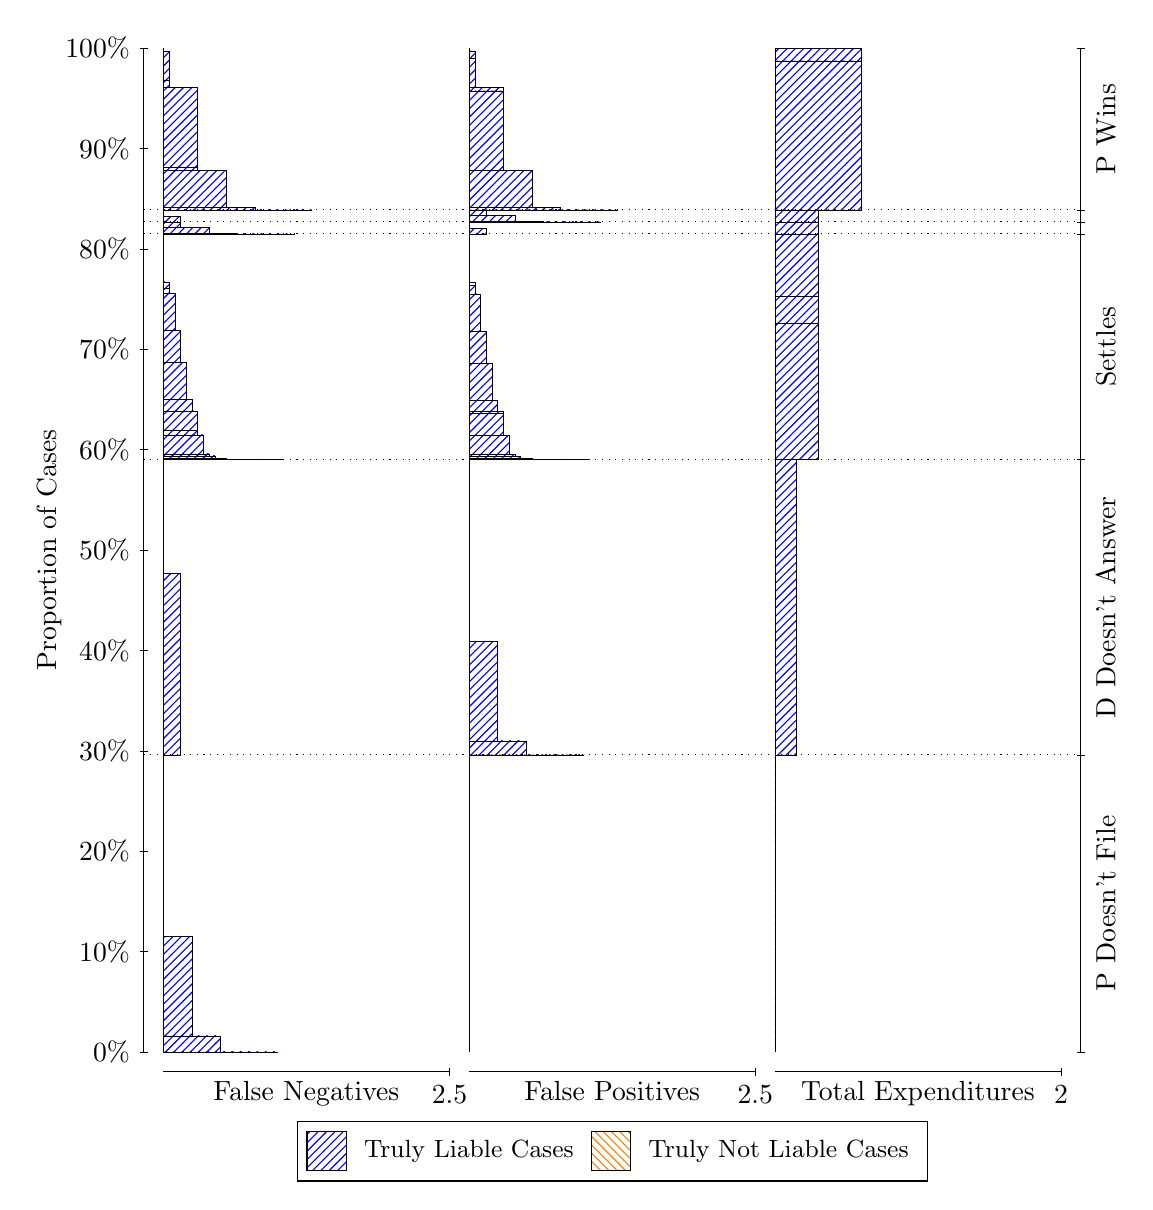
\begin{tikzpicture}
\draw[black, very thin] (1.5,1.75) -- (1.5,14.5);
\node[rotate=90, text=black, anchor=center] at (0.3, 8.125) {Proportion of Cases};
\draw[black, very thin] (1.45,1.75) -- (1.55,1.75);
\node[text=black, anchor=east] at (1.45, 1.75) {0\%};
\draw[black, very thin] (1.45,3.025) -- (1.55,3.025);
\node[text=black, anchor=east] at (1.45, 3.025) {10\%};
\draw[black, very thin] (1.45,4.3) -- (1.55,4.3);
\node[text=black, anchor=east] at (1.45, 4.3) {20\%};
\draw[black, very thin] (1.45,5.575) -- (1.55,5.575);
\node[text=black, anchor=east] at (1.45, 5.575) {30\%};
\draw[black, very thin] (1.45,6.85) -- (1.55,6.85);
\node[text=black, anchor=east] at (1.45, 6.85) {40\%};
\draw[black, very thin] (1.45,8.125) -- (1.55,8.125);
\node[text=black, anchor=east] at (1.45, 8.125) {50\%};
\draw[black, very thin] (1.45,9.4) -- (1.55,9.4);
\node[text=black, anchor=east] at (1.45, 9.4) {60\%};
\draw[black, very thin] (1.45,10.675) -- (1.55,10.675);
\node[text=black, anchor=east] at (1.45, 10.675) {70\%};
\draw[black, very thin] (1.45,11.95) -- (1.55,11.95);
\node[text=black, anchor=east] at (1.45, 11.95) {80\%};
\draw[black, very thin] (1.45,13.225) -- (1.55,13.225);
\node[text=black, anchor=east] at (1.45, 13.225) {90\%};
\draw[black, very thin] (1.45,14.5) -- (1.55,14.5);
\node[text=black, anchor=east] at (1.45, 14.5) {100\%};

\draw[black, very thin] (13.4,1.75) -- (13.4,14.5);
\draw[black, very thin] (13.35,1.75) -- (13.45,1.75);
\node[anchor=west] at (13.35, 1.75) {};
\draw[black, very thin] (13.35,5.5228) -- (13.45,5.5228);
\node[anchor=west] at (13.35, 5.5228) {};
\draw[black, very thin] (13.35,9.271) -- (13.45,9.271);
\node[anchor=west] at (13.35, 9.271) {};
\draw[black, very thin] (13.35,12.14) -- (13.45,12.14);
\node[anchor=west] at (13.35, 12.14) {};
\draw[black, very thin] (13.35,12.292) -- (13.45,12.292);
\node[anchor=west] at (13.35, 12.292) {};
\draw[black, very thin] (13.35,12.444) -- (13.45,12.444);
\node[anchor=west] at (13.35, 12.444) {};
\draw[black, very thin] (13.35,14.5) -- (13.45,14.5);
\node[anchor=west] at (13.35, 14.5) {};

\draw[black, very thin, pattern color=blue, pattern=north east lines] (1.75,1.75) rectangle (3.2033,1.75);
\draw[black, very thin, pattern color=blue, pattern=north east lines] (1.75,1.75) rectangle (2.84,1.7517);
\draw[black, very thin, pattern color=blue, pattern=north east lines] (1.75,1.7517) rectangle (2.4767,1.9536);
\draw[black, very thin, pattern color=blue, pattern=north east lines] (1.75,1.9536) rectangle (2.1133,3.2178);
\draw[black, very thin, pattern color=orange, pattern=north west lines] (1.75,3.2178) rectangle (1.75,3.2178);
\draw[black, very thin, pattern color=blue, pattern=north east lines] (1.75,3.2178) rectangle (1.75,5.5228);
\draw[black, very thin, pattern color=blue, pattern=north east lines] (1.75,5.5228) rectangle (1.968,7.8282);
\draw[black, very thin, pattern color=orange, pattern=north west lines] (1.75,7.8282) rectangle (1.75,7.8282);
\draw[black, very thin, pattern color=blue, pattern=north east lines] (1.75,7.8282) rectangle (1.75,9.271);
\draw[black, very thin, pattern color=blue, pattern=north east lines] (1.75,9.271) rectangle (3.276,9.271);
\draw[black, very thin, pattern color=blue, pattern=north east lines] (1.75,9.271) rectangle (2.9853,9.271);
\draw[black, very thin, pattern color=blue, pattern=north east lines] (1.75,9.271) rectangle (2.9127,9.271);
\draw[black, very thin, pattern color=blue, pattern=north east lines] (1.75,9.271) rectangle (2.84,9.271);
\draw[black, very thin, pattern color=blue, pattern=north east lines] (1.75,9.271) rectangle (2.6947,9.271);
\draw[black, very thin, pattern color=blue, pattern=north east lines] (1.75,9.271) rectangle (2.622,9.2774);
\draw[black, very thin, pattern color=blue, pattern=north east lines] (1.75,9.2774) rectangle (2.5493,9.2913);
\draw[black, very thin, pattern color=blue, pattern=north east lines] (1.75,9.2913) rectangle (2.4767,9.2918);
\draw[black, very thin, pattern color=blue, pattern=north east lines] (1.75,9.2918) rectangle (2.404,9.3189);
\draw[black, very thin, pattern color=blue, pattern=north east lines] (1.75,9.3189) rectangle (2.3313,9.3464);
\draw[black, very thin, pattern color=blue, pattern=north east lines] (1.75,9.3464) rectangle (2.2587,9.5872);
\draw[black, very thin, pattern color=blue, pattern=north east lines] (1.75,9.5872) rectangle (2.186,9.6413);
\draw[black, very thin, pattern color=blue, pattern=north east lines] (1.75,9.6413) rectangle (2.186,9.8909);
\draw[black, very thin, pattern color=blue, pattern=north east lines] (1.75,9.8909) rectangle (2.1133,10.034);
\draw[black, very thin, pattern color=blue, pattern=north east lines] (1.75,10.034) rectangle (2.0407,10.504);
\draw[black, very thin, pattern color=blue, pattern=north east lines] (1.75,10.504) rectangle (1.968,10.918);
\draw[black, very thin, pattern color=blue, pattern=north east lines] (1.75,10.918) rectangle (1.8953,11.385);
\draw[black, very thin, pattern color=blue, pattern=north east lines] (1.75,11.385) rectangle (1.8227,11.447);
\draw[black, very thin, pattern color=blue, pattern=north east lines] (1.75,11.447) rectangle (1.8227,11.529);
\draw[black, very thin, pattern color=blue, pattern=north east lines] (1.75,11.529) rectangle (1.75,11.552);
\draw[black, very thin, pattern color=orange, pattern=north west lines] (1.75,11.552) rectangle (1.75,11.552);
\draw[black, very thin, pattern color=blue, pattern=north east lines] (1.75,11.552) rectangle (1.75,12.14);
\draw[black, very thin, pattern color=blue, pattern=north east lines] (1.75,12.14) rectangle (3.4213,12.14);
\draw[black, very thin, pattern color=blue, pattern=north east lines] (1.75,12.14) rectangle (3.058,12.14);
\draw[black, very thin, pattern color=blue, pattern=north east lines] (1.75,12.14) rectangle (2.6947,12.142);
\draw[black, very thin, pattern color=blue, pattern=north east lines] (1.75,12.142) rectangle (2.3313,12.219);
\draw[black, very thin, pattern color=blue, pattern=north east lines] (1.75,12.219) rectangle (1.968,12.292);
\draw[black, very thin, pattern color=orange, pattern=north west lines] (1.75,12.292) rectangle (1.75,12.292);
\draw[black, very thin, pattern color=blue, pattern=north east lines] (1.75,12.292) rectangle (1.968,12.366);
\draw[black, very thin, pattern color=orange, pattern=north west lines] (1.75,12.366) rectangle (1.75,12.366);
\draw[black, very thin, pattern color=blue, pattern=north east lines] (1.75,12.366) rectangle (1.75,12.444);
\draw[black, very thin, pattern color=blue, pattern=north east lines] (1.75,12.444) rectangle (3.6393,12.444);
\draw[black, very thin, pattern color=blue, pattern=north east lines] (1.75,12.444) rectangle (3.276,12.444);
\draw[black, very thin, pattern color=blue, pattern=north east lines] (1.75,12.444) rectangle (2.9127,12.481);
\draw[black, very thin, pattern color=blue, pattern=north east lines] (1.75,12.481) rectangle (2.5493,12.948);
\draw[black, very thin, pattern color=blue, pattern=north east lines] (1.75,12.948) rectangle (2.186,12.99);
\draw[black, very thin, pattern color=blue, pattern=north east lines] (1.75,12.99) rectangle (2.186,13.996);
\draw[black, very thin, pattern color=blue, pattern=north east lines] (1.75,13.996) rectangle (1.8227,14.091);
\draw[black, very thin, pattern color=blue, pattern=north east lines] (1.75,14.091) rectangle (1.8227,14.464);
\draw[black, very thin, pattern color=orange, pattern=north west lines] (1.75,14.464) rectangle (1.75,14.464);
\draw[black, very thin, pattern color=blue, pattern=north east lines] (1.75,14.464) rectangle (1.75,14.5);
\draw[black, very thin, pattern color=orange, pattern=north west lines] (5.6333,1.75) rectangle (5.6333,1.75);
\draw[black, very thin, pattern color=blue, pattern=north east lines] (5.6333,1.75) rectangle (5.6333,5.5228);
\draw[black, very thin, pattern color=orange, pattern=north west lines] (5.6333,5.5228) rectangle (7.0867,5.5228);
\draw[black, very thin, pattern color=blue, pattern=north east lines] (5.6333,5.5228) rectangle (7.0867,5.5228);
\draw[black, very thin, pattern color=blue, pattern=north east lines] (5.6333,5.5228) rectangle (6.7233,5.5234);
\draw[black, very thin, pattern color=blue, pattern=north east lines] (5.6333,5.5234) rectangle (6.36,5.701);
\draw[black, very thin, pattern color=blue, pattern=north east lines] (5.6333,5.701) rectangle (5.9967,6.9656);
\draw[black, very thin, pattern color=blue, pattern=north east lines] (5.6333,6.9656) rectangle (5.6333,9.271);
\draw[black, very thin, pattern color=orange, pattern=north west lines] (5.6333,9.271) rectangle (7.1593,9.271);
\draw[black, very thin, pattern color=blue, pattern=north east lines] (5.6333,9.271) rectangle (7.1593,9.271);
\draw[black, very thin, pattern color=orange, pattern=north west lines] (5.6333,9.271) rectangle (6.8687,9.271);
\draw[black, very thin, pattern color=blue, pattern=north east lines] (5.6333,9.271) rectangle (6.8687,9.271);
\draw[black, very thin, pattern color=blue, pattern=north east lines] (5.6333,9.271) rectangle (6.796,9.271);
\draw[black, very thin, pattern color=orange, pattern=north west lines] (5.6333,9.271) rectangle (6.7233,9.271);
\draw[black, very thin, pattern color=blue, pattern=north east lines] (5.6333,9.271) rectangle (6.7233,9.271);
\draw[black, very thin, pattern color=orange, pattern=north west lines] (5.6333,9.271) rectangle (6.578,9.271);
\draw[black, very thin, pattern color=blue, pattern=north east lines] (5.6333,9.271) rectangle (6.578,9.271);
\draw[black, very thin, pattern color=blue, pattern=north east lines] (5.6333,9.271) rectangle (6.5053,9.2774);
\draw[black, very thin, pattern color=orange, pattern=north west lines] (5.6333,9.2774) rectangle (6.4327,9.2774);
\draw[black, very thin, pattern color=blue, pattern=north east lines] (5.6333,9.2774) rectangle (6.4327,9.2909);
\draw[black, very thin, pattern color=orange, pattern=north west lines] (5.6333,9.2909) rectangle (6.4327,9.2909);
\draw[black, very thin, pattern color=blue, pattern=north east lines] (5.6333,9.2909) rectangle (6.4327,9.291);
\draw[black, very thin, pattern color=blue, pattern=north east lines] (5.6333,9.291) rectangle (6.36,9.2914);
\draw[black, very thin, pattern color=orange, pattern=north west lines] (5.6333,9.2914) rectangle (6.2873,9.2914);
\draw[black, very thin, pattern color=blue, pattern=north east lines] (5.6333,9.2914) rectangle (6.2873,9.3183);
\draw[black, very thin, pattern color=blue, pattern=north east lines] (5.6333,9.3183) rectangle (6.2147,9.3435);
\draw[black, very thin, pattern color=blue, pattern=north east lines] (5.6333,9.3435) rectangle (6.142,9.5837);
\draw[black, very thin, pattern color=blue, pattern=north east lines] (5.6333,9.5837) rectangle (6.0693,9.859);
\draw[black, very thin, pattern color=blue, pattern=north east lines] (5.6333,9.859) rectangle (6.0693,9.8825);
\draw[black, very thin, pattern color=orange, pattern=north west lines] (5.6333,9.8825) rectangle (5.9967,9.8825);
\draw[black, very thin, pattern color=blue, pattern=north east lines] (5.6333,9.8825) rectangle (5.9967,10.026);
\draw[black, very thin, pattern color=blue, pattern=north east lines] (5.6333,10.026) rectangle (5.924,10.493);
\draw[black, very thin, pattern color=blue, pattern=north east lines] (5.6333,10.493) rectangle (5.8513,10.907);
\draw[black, very thin, pattern color=blue, pattern=north east lines] (5.6333,10.907) rectangle (5.7787,11.378);
\draw[black, very thin, pattern color=blue, pattern=north east lines] (5.6333,11.378) rectangle (5.706,11.489);
\draw[black, very thin, pattern color=blue, pattern=north east lines] (5.6333,11.489) rectangle (5.706,11.52);
\draw[black, very thin, pattern color=blue, pattern=north east lines] (5.6333,11.52) rectangle (5.6333,12.14);
\draw[black, very thin, pattern color=orange, pattern=north west lines] (5.6333,12.14) rectangle (5.8513,12.14);
\draw[black, very thin, pattern color=blue, pattern=north east lines] (5.6333,12.14) rectangle (5.8513,12.214);
\draw[black, very thin, pattern color=blue, pattern=north east lines] (5.6333,12.214) rectangle (5.6333,12.292);
\draw[black, very thin, pattern color=orange, pattern=north west lines] (5.6333,12.292) rectangle (7.3047,12.292);
\draw[black, very thin, pattern color=blue, pattern=north east lines] (5.6333,12.292) rectangle (7.3047,12.292);
\draw[black, very thin, pattern color=blue, pattern=north east lines] (5.6333,12.292) rectangle (6.9413,12.292);
\draw[black, very thin, pattern color=blue, pattern=north east lines] (5.6333,12.292) rectangle (6.578,12.294);
\draw[black, very thin, pattern color=blue, pattern=north east lines] (5.6333,12.294) rectangle (6.2147,12.371);
\draw[black, very thin, pattern color=blue, pattern=north east lines] (5.6333,12.371) rectangle (5.8513,12.444);
\draw[black, very thin, pattern color=orange, pattern=north west lines] (5.6333,12.444) rectangle (7.5227,12.444);
\draw[black, very thin, pattern color=blue, pattern=north east lines] (5.6333,12.444) rectangle (7.5227,12.444);
\draw[black, very thin, pattern color=orange, pattern=north west lines] (5.6333,12.444) rectangle (7.1593,12.444);
\draw[black, very thin, pattern color=blue, pattern=north east lines] (5.6333,12.444) rectangle (7.1593,12.444);
\draw[black, very thin, pattern color=orange, pattern=north west lines] (5.6333,12.444) rectangle (6.796,12.444);
\draw[black, very thin, pattern color=blue, pattern=north east lines] (5.6333,12.444) rectangle (6.796,12.481);
\draw[black, very thin, pattern color=orange, pattern=north west lines] (5.6333,12.481) rectangle (6.4327,12.481);
\draw[black, very thin, pattern color=blue, pattern=north east lines] (5.6333,12.481) rectangle (6.4327,12.948);
\draw[black, very thin, pattern color=blue, pattern=north east lines] (5.6333,12.948) rectangle (6.0693,13.955);
\draw[black, very thin, pattern color=orange, pattern=north west lines] (5.6333,13.955) rectangle (6.0693,13.955);
\draw[black, very thin, pattern color=blue, pattern=north east lines] (5.6333,13.955) rectangle (6.0693,13.996);
\draw[black, very thin, pattern color=blue, pattern=north east lines] (5.6333,13.996) rectangle (5.706,14.368);
\draw[black, very thin, pattern color=blue, pattern=north east lines] (5.6333,14.368) rectangle (5.706,14.464);
\draw[black, very thin, pattern color=blue, pattern=north east lines] (5.6333,14.464) rectangle (5.6333,14.5);
\draw[black, very thin, pattern color=orange, pattern=north west lines] (9.5167,1.75) rectangle (9.5167,1.75);
\draw[black, very thin, pattern color=blue, pattern=north east lines] (9.5167,1.75) rectangle (9.5167,5.5228);
\draw[black, very thin, pattern color=orange, pattern=north west lines] (9.5167,5.5228) rectangle (9.7892,5.5228);
\draw[black, very thin, pattern color=blue, pattern=north east lines] (9.5167,5.5228) rectangle (9.7892,9.271);
\draw[black, very thin, pattern color=orange, pattern=north west lines] (9.5167,9.271) rectangle (10.062,9.271);
\draw[black, very thin, pattern color=blue, pattern=north east lines] (9.5167,9.271) rectangle (10.062,10.999);
\draw[black, very thin, pattern color=orange, pattern=north west lines] (9.5167,10.999) rectangle (10.062,10.999);
\draw[black, very thin, pattern color=blue, pattern=north east lines] (9.5167,10.999) rectangle (10.062,11.343);
\draw[black, very thin, pattern color=orange, pattern=north west lines] (9.5167,11.343) rectangle (10.062,11.343);
\draw[black, very thin, pattern color=blue, pattern=north east lines] (9.5167,11.343) rectangle (10.062,12.14);
\draw[black, very thin, pattern color=orange, pattern=north west lines] (9.5167,12.14) rectangle (10.062,12.14);
\draw[black, very thin, pattern color=blue, pattern=north east lines] (9.5167,12.14) rectangle (10.062,12.292);
\draw[black, very thin, pattern color=orange, pattern=north west lines] (9.5167,12.292) rectangle (10.062,12.292);
\draw[black, very thin, pattern color=blue, pattern=north east lines] (9.5167,12.292) rectangle (10.062,12.444);
\draw[black, very thin, pattern color=orange, pattern=north west lines] (9.5167,12.444) rectangle (10.607,12.444);
\draw[black, very thin, pattern color=blue, pattern=north east lines] (9.5167,12.444) rectangle (10.607,14.338);
\draw[black, very thin, pattern color=orange, pattern=north west lines] (9.5167,14.338) rectangle (10.607,14.338);
\draw[black, very thin, pattern color=blue, pattern=north east lines] (9.5167,14.338) rectangle (10.607,14.5);
\draw[black, dotted] (1.5,5.5228) -- (13.4,5.5228);
\draw[black, dotted] (1.5,9.271) -- (13.4,9.271);
\draw[black, dotted] (1.5,12.14) -- (13.4,12.14);
\draw[black, dotted] (1.5,12.292) -- (13.4,12.292);
\draw[black, dotted] (1.5,12.444) -- (13.4,12.444);
\draw[black, very thin] (1.75,1.5) -- (5.3833,1.5);
\node[text=black, anchor=north] at (3.5667, 1.5) {False Negatives};
\draw[black, very thin] (5.3833,1.45) -- (5.3833,1.55);
\node[text=black, anchor=north] at (5.3833, 1.45) {2.5};

\draw[black, very thin] (5.6333,1.5) -- (9.2667,1.5);
\node[text=black, anchor=north] at (7.45, 1.5) {False Positives};
\draw[black, very thin] (9.2667,1.45) -- (9.2667,1.55);
\node[text=black, anchor=north] at (9.2667, 1.45) {2.5};

\draw[black, very thin] (9.5167,1.5) -- (13.15,1.5);
\node[text=black, anchor=north] at (11.333, 1.5) {Total Expenditures};
\draw[black, very thin] (13.15,1.45) -- (13.15,1.55);
\node[text=black, anchor=north] at (13.15, 1.45) {2};

\node[text=black, centered, rotate=90] at (13.72, 3.6364) {P Doesn't File};
\node[text=black, centered, rotate=90] at (13.72, 7.3969) {D Doesn't Answer};
\node[text=black, centered, rotate=90] at (13.72, 10.706) {Settles};


\node[text=black, centered, rotate=90] at (13.72, 13.472) {P Wins};

\draw (7.449999999999999,1.5) node[draw=none] (baseCoordinate) {};
\begin{scope}[align=center]
        \matrix[scale=0.5, draw=black, below=0.5cm of baseCoordinate, nodes={draw}, column sep=0.1cm]{
            \node[rectangle, draw, minimum width=0.5cm, minimum height=0.5cm, pattern color=blue, pattern=north east lines] {}; &
            \node[draw=none, font=\small, text=black] (B) {Truly Liable Cases}; &
            \node[rectangle, draw, minimum width=0.5cm, minimum height=0.5cm, pattern color=orange, pattern=north west lines] {}; &
            \node[draw=none, font=\small, text=black] (B) {Truly Not Liable Cases}; \\
            };
\end{scope}

\end{tikzpicture}
\end{document}